%% For double-blind review submission, w/o CCS and ACM Reference (max submission space)
\documentclass[10pt, sigplan]{acmart}
%%\settopmatter{printfolios=true,printccs=false,printacmref=false}
%% For double-blind review submission, w/ CCS and ACM Reference
%\documentclass[sigplan,10pt,review,anonymous]{acmart}\settopmatter{printfolios=true}
%% For single-blind review submission, w/o CCS and ACM Reference (max submission space)
%\documentclass[sigplan,10pt,review]{acmart}\settopmatter{printfolios=true,printccs=false,printacmref=false}
%% For single-blind review submission, w/ CCS and ACM Reference
%\documentclass[sigplan,10pt,review]{acmart}\settopmatter{printfolios=true}
%% For final camera-ready submission, w/ required CCS and ACM Reference
%\documentclass[sigplan,10pt]{acmart}\settopmatter{}


%% Conference information
%% Supplied to authors by publisher for camera-ready submission;
%% use defaults for review submission.
%\acmConference[PL'17]{ACM SIGPLAN Conference on Programming Languages}{January 01--03, 2017}{New York, NY, USA}
%\acmYear{2017}
%\acmISBN{} % \acmISBN{978-x-xxxx-xxxx-x/YY/MM}
%\acmDOI{} % \acmDOI{10.1145/nnnnnnn.nnnnnnn}
%\startPage{1}

%% Copyright information
%% Supplied to authors (based on authors' rights management selection;
%% see authors.acm.org) by publisher for camera-ready submission;
%% use 'none' for review submission.
\setcopyright{none}
%\setcopyright{acmcopyright}
%\setcopyright{acmlicensed}
%\setcopyright{rightsretained}
%\copyrightyear{2017}           %% If different from \acmYear

%% Bibliography style
%%\bibliographystyle{ACM-Reference-Format}
%% Citation style
%\citestyle{acmauthoryear}  %% For author/year citations
%\citestyle{acmnumeric}     %% For numeric citations
%\setcitestyle{nosort}      %% With 'acmnumeric', to disable automatic
                            %% sorting of references within a single citation;
                            %% e.g., \cite{Smith99,Carpenter05,Baker12}
                            %% rendered as [14,5,2] rather than [2,5,14].
%\setcitesyle{nocompress}   %% With 'acmnumeric', to disable automatic
                            %% compression of sequential references within a
                            %% single citation;
                            %% e.g., \cite{Baker12,Baker14,Baker16}
                            %% rendered as [2,3,4] rather than [2-4].


%%%%%%%%%%%%%%%%%%%%%%%%%%%%%%%%%%%%%%%%%%%%%%%%%%%%%%%%%%%%%%%%%%%%%%
%% Note: Authors migrating a paper from traditional SIGPLAN
%% proceedings format to PACMPL format must update the
%% '\documentclass' and topmatter commands above; see
%% 'acmart-pacmpl-template.tex'.
%%%%%%%%%%%%%%%%%%%%%%%%%%%%%%%%%%%%%%%%%%%%%%%%%%%%%%%%%%%%%%%%%%%%%%


%% Some recommended packages.
\usepackage{booktabs}   %% For formal tables:
                        %% http://ctan.org/pkg/booktabs
\usepackage{subcaption} %% For complex figures with subfigures/subcaptions
                        %% http://ctan.org/pkg/subcaption
\usepackage{xspace}
\usepackage{graphicx}
\usepackage{ifthen}
%



% Source Code
%\usepackage{color}
%\usepackage{textcomp}
%\usepackage{listings}
%\usepackage{ulem}
%\usepackage[T1]{fontenc}
%\usepackage{times}
% \usepackage{needspace}
 

% Source Code
\usepackage{color}
\usepackage{textcomp}
\usepackage{listings}

\definecolor{source}{gray}{0.85}% my comment style
\newcommand{\myCommentStyle}[1]{{\footnotesize\sffamily\color{gray!100!white} #1}}
%\newcommand{\myCommentStyle}[1]{{\footnotesize\sffamily\color{black!100!white} #1}}

% my string style
\newcommand{\myStringStyle}[1]{{\footnotesize\sffamily\color{violet!100!black} #1}}
%\newcommand{\myStringStyle}[1]{{\footnotesize\sffamily\color{black!100!black} #1}}

% my symbol style
\newcommand{\mySymbolStyle}[1]{{\footnotesize\sffamily\color{violet!100!black} #1}}
%\newcommand{\mySymbolStyle}[1]{{\footnotesize\sffamily\color{black!100!black} #1}}

% my keyword style
\newcommand{\myKeywordStyle}[1]{{\footnotesize\sffamily\color{green!70!black} #1}}
%\newcommand{\myKeywordStyle}[1]{{\footnotesize\sffamily\color{black!70!black} #1}}

% my global style
\newcommand{\myGlobalStyle}[1]{{\footnotesize\sffamily\color{blue!100!black} #1}}
%\newcommand{\myGlobalStyle}[1]{{\footnotesize\sffamily\color{black!100!black} #1}}

% my number style
\newcommand{\myNumberStyle}[1]{{\footnotesize\sffamily\color{brown!100!black} #1}}
%\newcommand{\myNumberStyle}[1]{{\footnotesize\sffamily\color{black!100!black} #1}}

\lstset{
language={},
% characters
tabsize=3,
escapechar={!},
keepspaces=true,
breaklines=true,
alsoletter={\#},
literate={\$}{{{\$}}}1,
breakautoindent=true,
columns=fullflexible,
showstringspaces=false,
% background
frame=single,
aboveskip=1em, % automatic space before
framerule=0pt,
basicstyle=\footnotesize\sffamily\color{black},
keywordstyle=\myKeywordStyle,% keyword style
commentstyle=\myCommentStyle,% comment style
frame=single,%
backgroundcolor=\color{source},
% numbering
stepnumber=1,
numbersep=10pt,
numberstyle=\tiny,
numberfirstline=true,
% caption
captionpos=b,
% formatting (html)
moredelim=[is][\bfseries]{<b>}{</b>},
moredelim=[is][\textit]{<i>}{</i>},
moredelim=[is][\underbar]{<u>}{</u>},
moredelim=[is][\color{red}\uwave]{<wave>}{</wave>},
moredelim=[is][\color{red}\sout]{<del>}{</del>},
moredelim=[is][\color{blue}\underbar]{<ins>}{</ins>},
% smalltalk stuff
morecomment=[s][\myCommentStyle]{"}{"},
%    morecomment=[s][\myvs]{|}{|},
morestring=[b][\myStringStyle]',
moredelim=[is][]{<sel>}{</sel>},
moredelim=[is][]{<rcv>}{</rcv>},
moredelim=[is][\itshape]{<symb>}{</symb>},
moredelim=[is][\scshape]{<class>}{</class>},
morekeywords={true,false,nil,self,super,thisContext},
identifierstyle=\idstyle,
}

\makeatletter
\newcommand*\idstyle[1]{%
\expandafter\id@style\the\lst@token{#1}\relax%
}
\def\id@style#1#2\relax{%
\ifnum\pdfstrcmp{#1}{\#}=0%
% this is a symbol
\mySymbolStyle{\the\lst@token}%
\else%
\edef\tempa{\uccode`#1}%
\edef\tempb{`#1}%
\ifnum\tempa=\tempb%
% this is a global
\myGlobalStyle{\the\lst@token}%
\else%
\the\lst@token%
\fi%
\fi%
}
\makeatother


%\newcommand{\ct}{\lstinline[backgroundcolor=\color{white}]}
%\newcommand{\needlines}[1]{\Needspace{#1\baselineskip}}
\newcommand{\lct}{\texttt}

\lstnewenvironment{code}{%
    \lstset{%
    % frame=lines,
    frame=single,
    framerule=0pt,
    mathescape=false
    }%
    \noindent%
    \minipage{\linewidth}%
}{%
    \endminipage%
}%


\lstnewenvironment{codeWithLineNumbers}{%
    \lstset{%
    % frame=lines,
    frame=single,
    framerule=0pt,
    mathescape=false,
    numbers=left
    }%
    \noindent%
    \minipage{\linewidth}%
}{%
    \endminipage%
}%



\newenvironment{codeNonSmalltalk}
{\begin{alltt}\sffamily}
{\end{alltt}\normalsize}



\usepackage{xcolor}
\newcommand{\sd}[1]{\color{red}\fbox{\bfseries\sffamily\scriptsize Stef:}{\sf\small$\blacktriangleright$\textit{#1}$\blacktriangleleft$}\color{black}}
\newcommand{\sk}[1]{\color{blue}\fbox{\bfseries\sffamily\scriptsize Sophie:}{\sf\small$\blacktriangleright$\textit{#1}$\blacktriangleleft$}\color{black}}
\newcommand{\cba}[1]{\color{purple}\fbox{\bfseries\sffamily\scriptsize Clement:}{\sf\small$\blacktriangleright$\textit{#1}$\blacktriangleleft$}\color{black}}


\begin{document}

%% Title information
\title[Short Title]{Assessing primitives performance\\ on multi-stage execution}       

%% Author with single affiliation.
\author{Sophie Kaleba}
                                        %% can be repeated if necessary
\affiliation{
  %\position{Position1}
  \department{RMoD}              %% \department is recommended
  \institution{Inria}            %% \institution is required
 % \streetaddress{Street1 Address1}
  \city{Lille}
  %\state{France}
  %\postcode{Post-Code1}
  \country{France}                    %% \country is recommended
}
\email{sophie.kaleba@etudiant.univ-lille1.fr}          %% \email is recommended

%% Author with two affiliations and emails.
\author{Cl\'ement B\'era}
\affiliation{
  % \position{}
	\department{Software Languages Lab}              %% \department is recommended
	\institution{Vrije Universiteit Brussel}            %% \institution is required
	\city{Brussel}
  % \state{}
  % \postcode{}
	\country{Belgium}                    %% \country is recommended
}
\email{clement.bera@vub.ac.be}          %% \email is recommended

%% Author with two affiliations and emails.
\author{St\'ephane Ducasse}
\affiliation{
 % \position{Position2b}
  \department{RMoD}             %% \department is recommended
  \institution{Inria}           %% \institution is required
  %\streetaddress{Street3b Address2b}
  \city{Lille}
  %\state{State2b}
  %\postcode{Post-Code2b}
  \country{France}                   %% \country is recommended
}
\email{stephane.ducasse@inria.fr}         %% \email is recommended


%% Abstract
%% Note: \begin{abstract}...\end{abstract} environment must come
%% before \maketitle command
\begin{abstract}

Virtual machines, besides the interpreter and just-in-time compiler optimization facilities, also include a set of primitive operations that the client language can use. Some of these are essential and cannot be performed in any other way. Others are optional, they can be expressed in the client language but are often implemented in the virtual machine to improve performance when the just-in-time compiler is unable to do so (start-up performance, speculative optimizations not implemented or not mature enough, etc.).

In a hybrid runtime, where code is executed by an interpreter and a just-in-time compiler, the implementor can choose to implement optional primitives in the client language, in the virtual machine implementation language (typically C or C++) or on top of the just-in-time compiler back-end. We implemented the String comparison optional primitive in each case. This paper describes the different implementations and compares the execution time in Cog, a Smalltalk virtual machine. 

The paper shows that the implementation with the most reliable and high performance is also the most complex and difficult to implement. Since hundreds of optional primitives can be available, the virtual machine implementor has to carefully choose how to implement each of them to balance between maintenance cost and high performance.

\end{abstract}

%% 2012 ACM Computing Classification System (CSS) concepts
%% Generate at 'http://dl.acm.org/ccs/ccs.cfm'.
%\begin{CCSXML}
%<ccs2012>
%<concept>
%<concept_id>10011007.10011006.10011008</concept_id>
%<concept_desc>Software and its engineering~General programming languages</concept_desc>
%<concept_significance>500</concept_significance>
%</concept>
%<concept>
%<concept_id>10003456.10003457.10003521.10003525</concept_id>
%<concept_desc>Social and professional topics~History of programming languages</concept_desc>
%<concept_significance>300</concept_significance>
%</concept>
%</ccs2012>
%\end{CCSXML}

%\ccsdesc[500]{Software and its engineering~General programming languages}
%\ccsdesc[300]{Social and professional topics~History of programming languages}
%% End of generated code


%% Keywords
%% comma separated list
\keywords{Just-in-Time compiler, Primitive, Virtual machine, Managed runtime}  %% \keywords are mandatory in final camera-ready submission


%% \maketitle
%% Note: \maketitle command must come after title commands, author
%% commands, abstract environment, Computing Classification System
%% environment and commands, and keywords command.
\maketitle


\section{Introduction}

%Managed lang

Dynamically typed programming languages are traditionally
implemented as virtual machines (VMs). As the popularity
of VM-based languages has increased, VM implementation
techniques have evolved to the point where most mature
VMs utilize some form of just-in-time (JIT) compilation, with
two main technologies contending at the moment: method
JITs [12], which generally compile methods at a time into
machine code, and utilize techniques such as inlining and
branch pruning to simplify the code or merge multiple methods;
and tracing JITs [1], which record the actions of the
program including branches taken and methods dispatched
into a specific trace and compile it into machine code

Define JIT VM acronym

\subsection{Primitive execution}

 prim, optional and essential MENTION built-in
 Il faut definir primitive, primitive essentielle, primitive d'optimisation. Il faut expliquer brievement les primitives Smalltalk, comment elles sont activ�es, dans quelles cas le fall back code est appel�, que si elles fail c'est side-effect free. => Dans mon papier ISMM'15 il y a une explication section 4.2 le d�but de Primitive operations. dont tu peux t'inspirer, voir copier coller comme je suis auteur des 2.

primitive performance: VM without opt JIT, before reaching peak perf, or jit incorrectly optimizing specific part of code.

\subsection{VM execution model}

Il faut expliquer le process de compilation de la VM. (Slang -> C, C-> ASM, au runtime JIT ST->ASM)
 execution with C and St stack

\begin{figure}[tb]
		\centering
		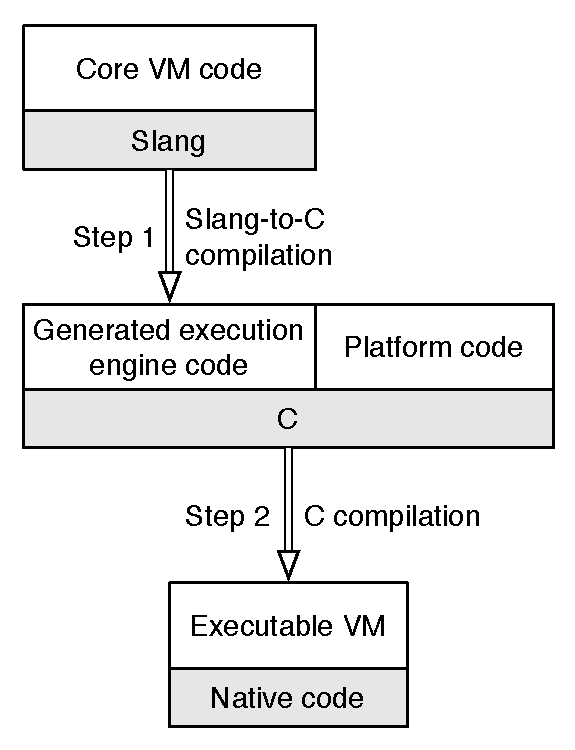
\includegraphics[width=0.6\linewidth]{figures/VMCompilation}
		\caption{VM compilation}
		\label{fig:VMCompilation}
\end{figure}

 Il faut que tu pr�cises bien le co�t de changement entre la pile St et la pile C et que tu expliques le probleme des primitives C courtes appel�es depuis le code g�n�r� par le JIT. Je ferais une figure. C'est important pour la suite. 

\subsection{String comparison primitive}

 Comme le coeur du papier est sur String prim, tu introduis la primitive sur laquelle tu vas travailler, dont la representation des strings, ses cas d'utilisation
 Short description of the String class (String, ByteString, WideString)?

\section{Different primitive implementations}
 
 \subsection{Context}
 
 [Max 1/2 page, justifie 1,2,3 et non neg,0,pos]
 
We had SmartSyntax primitive.
Explain 1,2,3 results
Problem compatibility other languages
expect neg,0,pos

Wanting to improve performance

2 critical problems:
(1) changing the prim => changing all clients (VM compil from Pharo or Squeak different results)
(2) no support in SmartSyntax for read-only objects. [plugins but not String comparison]

Premiere tentative Eliot -> Slang plugin. Keep 1,2,3. Resoud Read-only / changing the prim problems.

Deuxieme tentative Slang internal, then Cog's RTL.
=> pour simplifier le RTL neg,0,pos etait mieux => minus instead of branches.
=> compat execution model, Slang internal neg,0, pos too.

 \subsection{Different implementation and execution}
 
- Pure Smalltalk: baseline
Smalltalk code on top of VM. Used as our baseline for benchmarks.
Write down the Smalltalk code here.
Expliquer to:do: over do: (to explain expresiveness) => core lib often use to:do: and not do:

- Smart Syntax Plugin
%= aString 	
%	self == aString ifTrue: [ ^true ].
%	aString isString ifFalse: [ ^false ].
%	self size = aString size ifFalse: [ ^false ].
%	1 to: self size do: [:i | (self at: i) = (aString at: i) ifFalse: [^false] ].
%	^ true
Restricted Smalltalk

written in Smalltalk with restrictions.
Compiled to C AOT into a plugin.

- Slang plugin 
Slang, but no access au fonctions de la VM drectement.
 interpreterProxy. (C compiler inlining, linking time ? cmacro ?)

- Slang pure

- Slang pure + Cog RTL

generate functions as machine code
partial implementation (frequent cases are implemented)
Sometimes, fallback to less-optimised version

 
 \subsection{Pros and cons}
 
  Can be changed like Smalltalk code (No C compilation whatsoever). Readability. Only impl without VM recompilation.

Baseline performance is not that great, jtted performance is good only with mature optimizing JIT we don't have.

Number of implementations: 1, 2 or 3: same implem for primitive in C and fall back code in Smalltalk, relatively easy to read/code.
recompilation. 
changing the prim => changing all clients (VM compil from Pharo or Squeak different results
Performance: cross file inlining not possible by default. (InterpreterProxy indirection)
Control on generated code => difference LLVM/GCC
 Pure C performance (no interpreter proxy).
 no C-St jump. Control over the outcome (reliable performance)
 costly jumps between Smalltalk and C runtime (trampolines), need to recompile vm sources, little control over outcome (c compilers 
 need to recompile vm sources (trampolines), code readability 
 
 \subsection{Comparison}


\cba{expliquer tableau comparatif}

Trade-off engineering time and performance.
- recompiler la VM ou pas (Plugin externes, code Smalltalk)
- complexite d'implem (comprehension Smalltalk, C, ASM)



%%%%%
% END OLD
%%%%%

\section{Evaluation}
All these versions of the primitives have been implemented. Compare performances

\subsection{Set-up}
Describe set-up:
GCC eval Ubuntu + machine spec
LLVM eval Mac OS X + machine spec.

\subsection{Micro-benchmarks}
Results on strings of different lengths (3, 10, 1000)

4 string length. (1er <=3, dernier > 1000) 
line 1: GCC
line 2: LLVM
String evaluation here.

\cba{Show ASM loops and discuss the differences
add appendix with full code}

\subsection{Macro-benchmarks}
JSON

\section{Related work}

\begin{itemize}
	%\item Java: platform dependent
	\item V8: interpreter compiled by JIT
	optimised backend
	as if we were compiling slang using the JIT compiler (ahead of time)
	no more virtual call
	\item VisualWorks: baseline JIT but no interpreter => only 1 implement to write and maintain.
	\item Self - Strongtalk -> tout en Smalltalk avec mature optimizing JIT. pb baseline perf, haut cout de maintenance implem pour l'adaptive optimizer
\end{itemize}

\cba{Ajoute le related work que tu as trouv� de ICOOOLPS avec le travail de Tim.}

\section{Future work and conclusion}
1. number of representations\\
2. common representation
\cba{Future work -> primitive processor dependent (i.e. SSE4 instrs), pros and cons and why you did not do it (ingeniering cost per back-end)}
\cba{Inlining in Sista + ref}

Conclusion: trade off expressiveness performance


%% Acknowledgments
%%\begin{acks}                            %% acks environment is optional
                                        %% contents suppressed with 'anonymous'
  %% Commands \grantsponsor{<sponsorID>}{<name>}{<url>} and
  %% \grantnum[<url>]{<sponsorID>}{<number>} should be used to
  %% acknowledge financial support and will be used by metadata
  %% extraction tools.
%  This material is based upon work supported by the
%  \grantsponsor{GS100000001}{National Science
%    Foundation}{http://dx.doi.org/10.13039/100000001} under Grant
%  No.~\grantnum{GS100000001}{nnnnnnn} and Grant
%  No.~\grantnum{GS100000001}{mmmmmmm}.  Any opinions, findings, and
%  conclusions or recommendations expressed in this material are those
%  of the author and do not necessarily reflect the views of the
%  National Science Foundation.
%\end{acks}


%% Bibliography
%\bibliography{bibfile}


%% Appendix
\appendix
\section{Appendix}

\cba{Source code et generated C and ASM code for all versions}

Text of appendix \ldots

\end{document}
